% Fibres of reduction modulo three: the map remembers a coset, not its representative.
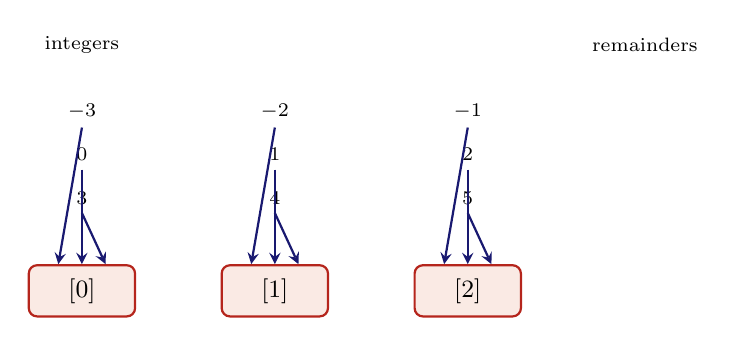
\begin{tikzpicture}[x=1cm,y=1cm,>=stealth,
 small/.style={font=\scriptsize,inner sep=3pt},
 bucket/.style={draw=BrickRed,rounded corners=3pt,thick,fill=BrickRed!7,minimum width=1.35cm,minimum height=.65cm,font=\small}]
\node[small] at (0,1.85) {integers};
\node[small] at (7.15,1.85) {remainders};
\foreach \x/\a/\bb/\c/\tag in {0/-3/0/3/0,2.45/-2/1/4/1,4.9/-1/2/5/2}{
  \node[small] (a\tag) at (\x,1) {$\a$};
  \node[small] (b\tag) at (\x,0.45) {$\bb$};
  \node[small] (c\tag) at (\x,-0.1) {$\c$};
  \node[bucket] (d\tag) at (\x,-1.28) {$[\tag]$};
  \draw[->,MidnightBlue,thick] (a\tag.south) -- ([xshift=-.3cm]d\tag.north);
  \draw[->,MidnightBlue,thick] (b\tag.south) -- (d\tag.north);
  \draw[->,MidnightBlue,thick] (c\tag.south) -- ([xshift=.3cm]d\tag.north);
}
\end{tikzpicture}
